\documentclass[12pt, a4paper]{article}

% ─── Packages ───────────────────────────────────────────────────────────────
\usepackage[margin=2.5cm]{geometry}
\usepackage{amsmath, amssymb, amsthm}
\usepackage{mathtools}
\usepackage{bm}
\usepackage{graphicx}
\usepackage{booktabs}
\usepackage{multirow}
\usepackage{array}
\usepackage{hyperref}
\usepackage{xcolor}
\usepackage{enumitem}
\usepackage{tcolorbox}
\usepackage{fancyhdr}
\usepackage{titlesec}
\usepackage{caption}
\usepackage{subcaption}
\usepackage{algorithm}
\usepackage{algpseudocode}
\usepackage{setspace}
\usepackage{nicefrac}
\usepackage{tikz}
\usetikzlibrary{arrows.meta, shapes.geometric, positioning, fit, backgrounds}

% ─── Colours ────────────────────────────────────────────────────────────────
\definecolor{thesisblue}{RGB}{31, 73, 125}
\definecolor{thesisgray}{RGB}{89, 89, 89}
\definecolor{donegreen}{RGB}{0, 128, 0}
\definecolor{inprogressorange}{RGB}{204, 102, 0}
\definecolor{plannedpurple}{RGB}{102, 0, 153}
\definecolor{lightblue}{RGB}{220, 235, 252}
\definecolor{lightgreen}{RGB}{220, 252, 230}
\definecolor{lightyellow}{RGB}{255, 253, 220}
\definecolor{lightpurple}{RGB}{240, 220, 255}
\definecolor{lightorange}{RGB}{255, 240, 220}
\definecolor{lightgray}{RGB}{245, 245, 245}
\definecolor{corered}{RGB}{180, 20, 20}

% ─── Hyperref ────────────────────────────────────────────────────────────────
\hypersetup{colorlinks=true,linkcolor=thesisblue,citecolor=thesisblue,
            urlcolor=thesisblue}

% ─── Headers ─────────────────────────────────────────────────────────────────
\pagestyle{fancy}\fancyhf{}
\rhead{\textcolor{thesisgray}{\small Cognitive Radar Beam Selection -- Thesis Anchor}}
\lhead{\textcolor{thesisgray}{\small \leftmark}}
\cfoot{\thepage}
\renewcommand{\headrulewidth}{0.4pt}

% ─── Section formatting ──────────────────────────────────────────────────────
\titleformat{\section}{\Large\bfseries\color{thesisblue}}{S\thesection}{1em}{}[\titlerule]
\titleformat{\subsection}{\large\bfseries\color{thesisblue}}{\thesubsection}{1em}{}
\titleformat{\subsubsection}{\normalsize\bfseries\color{thesisgray}}{\thesubsubsection}{1em}{}

% ─── Custom boxes ────────────────────────────────────────────────────────────
\newtcolorbox{donebox}{colback=lightgreen,colframe=donegreen,
  fonttitle=\bfseries,title={\checkmark\ COMPLETED}}
\newtcolorbox{nextbox}{colback=lightyellow,colframe=inprogressorange,
  fonttitle=\bfseries,title={NEXT STEP}}
\newtcolorbox{futurebox}{colback=lightpurple,colframe=plannedpurple,
  fonttitle=\bfseries,title={FUTURE STEP}}
\newtcolorbox{notebox}{colback=lightblue,colframe=thesisblue,
  fonttitle=\bfseries,title={Note}}
\newtcolorbox{plainbox}{colback=lightgray,colframe=thesisgray,
  fonttitle=\bfseries,title={Plain English}}
\newtcolorbox{corebox}{colback=lightorange,colframe=corered,
  fonttitle=\bfseries\color{white},colbacktitle=corered,
  title={CORE CONTRIBUTION}}
\newtcolorbox{ablationbox}{colback=lightpurple,colframe=plannedpurple,
  fonttitle=\bfseries,title={ABLATION STUDY}}

% ─── Math macros ─────────────────────────────────────────────────────────────
\DeclareMathOperator*{\argmax}{arg\,max}
\DeclareMathOperator*{\argmin}{arg\,min}
\newcommand{\Hent}{\mathcal{H}}
\newcommand{\beam}{\mathcal{B}}
\newcommand{\beamset}{\mathcal{S}}
\newcommand{\bev}{\mathrm{BEV}}
\newcommand{\pv}{\mathrm{PV}}
\newcommand{\fv}{\mathrm{FV}}
\newcommand{\DI}{\mathbf{D}_{I}}
\newcommand{\CI}{\mathbf{C}_{I}}
\newcommand{\CR}{\mathbf{C}_{R}}
\newcommand{\OR}{\mathbf{O}_{R}}
\newcommand{\FI}{\mathbf{F}_{I}}
\newcommand{\Fbev}{\mathbf{F}^{\bev}}
\newcommand{\Udep}{U_{\mathrm{depth}}}
\newcommand{\Uatt}{U_{\mathrm{attn}}}
\newcommand{\Uout}{U_{\mathrm{out}}}
\newcommand{\E}{\mathbb{E}}
\newcommand{\Var}{\mathrm{Var}}
\newcommand{\R}{\mathbb{R}}

% ─── Theorem environments ────────────────────────────────────────────────────
\theoremstyle{definition}
\newtheorem{definition}{Definition}[section]
\newtheorem{proposition}{Proposition}[section]
\newtheorem{remark}{Remark}[section]

\setstretch{1.2}
\setlength{\parskip}{4pt}

% =============================================================================
\begin{document}
% =============================================================================

\begin{titlepage}
  \centering\vspace*{1.8cm}
  {\color{thesisblue}\rule{\linewidth}{1.5pt}}\\[0.5cm]
  {\Huge\bfseries\color{thesisblue}
    Cognitive Radar Beam Selection\\[0.35cm]
    via Perceptual Uncertainty\\[0.35cm]
    in Autonomous Driving}\\[0.5cm]
  {\color{thesisblue}\rule{\linewidth}{1.5pt}}\\[1.2cm]
  {\LARGE\bfseries Thesis Anchor Document}\\[0.35cm]
  {\large\color{thesisgray}
    Architecture, mathematics, plain-English explanations, status, roadmap}\\[1.8cm]
  \begin{tabular}{rl}
    \textbf{Candidate:}     & [Your Name]               \\[4pt]
    \textbf{Supervisor:}    & [Supervisor Name]          \\[4pt]
    \textbf{Institution:}   & [University / Department]  \\[4pt]
    \textbf{Last updated:}  & \today                     \\
  \end{tabular}
  \vfill
  {\small\color{thesisgray}
    Single source of truth for the thesis. Update after every major experiment.}
\end{titlepage}

\tableofcontents\newpage

% =============================================================================
\section{Thesis Overview and Core Idea}
\label{sec:overview}
% =============================================================================

\subsection{The Problem in Plain English}

\begin{plainbox}
A radar on a car normally scans every direction at every moment, whether or not
there is anything interesting in those directions.
This wastes power and limits how fast the radar can scan important areas.

The question this thesis asks is: \textbf{can the camera tell the radar where
to look?} Instead of scanning everywhere, can the car look at its camera images,
figure out which directions are uncertain or interesting, and only fire radar beams
in those directions?

This is the idea of \emph{cognitive radar} applied to autonomous driving: a
sensing system that adapts what it measures based on what it already perceives.
\end{plainbox}

\subsection{Core Research Question}

Given only camera images at time $t$, find the subset of radar beams
$\beamset \subseteq \{\beam_1,\ldots,\beam_{N_B}\}$ of size $K = \lfloor\alpha N_B\rfloor$
that maximises 3D detection performance when those beams are transmitted:
\begin{equation}
  \beamset^*_\alpha
  \;=\;
  \argmax_{\beamset,\,|\beamset|=K}
  \;\mathrm{mAP}\!\left(\mathbf{I},\,\mathcal{R}(\beamset)\right)
  \label{eq:problem}
\end{equation}
where $\mathcal{R}(\beamset)$ is the radar point cloud restricted to selected beams.

\subsection{What is Core and What is Ablation}
\label{sec:core_vs_ablation}

It is important to be explicit about what this thesis claims as its main
contribution and what is exploratory.

\begin{corebox}
\textbf{The core contribution of this thesis is:}
\begin{enumerate}
  \item Demonstrating that camera-derived \textbf{perceptual uncertainty} is a
        valid and effective proxy for radar beam utility, outperforming
        random and uniform beam selection at every beam budget.
  \item Proposing and validating a concrete pipeline that runs the camera model
        first, computes uncertainty, selects beams, and then fires the radar ---
        a causally valid closed-loop cognitive radar system.
  \item Showing that a small fraction $\alpha^*$ of beams suffices to recover
        $\geq 99\%$ of full-scan detection performance, quantifying the
        power saving achievable.
\end{enumerate}
The \textbf{primary uncertainty signal} used throughout is the \textbf{output
detection entropy from the camera-only CRN ensemble} (Phase~2-A).
\end{corebox}

\begin{ablationbox}
\textbf{Ablation studies} explore secondary questions that strengthen the paper
but are not the main claim:
\begin{itemize}
  \item Total entropy vs.\ epistemic-only entropy as beam score
  \item Depth distribution entropy (Phase~2-B) vs.\ output entropy
  \item MFA attention weights (Phase~2-C) as an alternative signal
  \item Beam width sensitivity ($\Delta\theta$)
  \item Weather and lighting breakdown
  \item Learned policy (Phase~3) vs.\ heuristic scoring
\end{itemize}
\end{ablationbox}

% =============================================================================
\section{The CRN Architecture --- A Thorough Walkthrough}
\label{sec:crn}
% =============================================================================

\begin{plainbox}
This section explains exactly what CRN does, step by step, in plain language
and then in math. Read the plain-language paragraph first before the equations.
\end{plainbox}

\subsection{What CRN is Trying to Do}

CRN takes as input: six camera images pointing in different directions around
the car, and a sparse radar point cloud. It outputs: a Bird's-Eye-View (BEV)
map of the scene from above, with predicted 3D bounding boxes for all objects.

The hard problem it solves is that cameras see the world in 2D (flat images)
but we need 3D information. The clever trick is to use the radar's accurate
distance measurements to help ``lift'' the camera images into 3D.

CRN does this in two stages:
\begin{enumerate}
  \item \textbf{RVT} --- use radar to help the camera figure out depth, then
        project everything into a top-down BEV map
  \item \textbf{MFA} --- intelligently merge the camera BEV map and radar BEV
        map into one unified representation
\end{enumerate}

\subsection{Stage 1: Radar-assisted View Transformation (RVT)}

\subsubsection{Step 1a: Extract image features}

\begin{plainbox}
The six camera images are fed through a neural network (ResNet backbone with FPN).
Think of this as the network ``reading'' the images and producing a rich feature
description of every pixel --- not just colour, but what kind of object might be
at that pixel, what texture it has, etc.
\end{plainbox}

\begin{equation}
  \FI = \mathrm{ResNet{+}FPN}(\{I_n\}_{n=1}^{6})
  \;\in\; \R^{N \times C \times H \times W}
\end{equation}

From these features, two quantities are extracted:

\paragraph{Image context features} (what is at each pixel):
\begin{equation}
  \CI^\pv = \mathrm{Conv}(\FI)
  \;\in\; \R^{N \times C \times H \times W}
\end{equation}

\paragraph{Depth distribution} (how far away is each pixel):
\begin{equation}
  \DI(u,v) = \mathrm{Softmax}\!\left(\mathrm{Conv}(\FI)(u,v)\right)
  \;\in\; \R^{N \times D \times H \times W}
  \label{eq:depth_dist}
\end{equation}

\begin{plainbox}
For every pixel $(u,v)$ in every camera, the network outputs a probability
distribution over $D = 112$ depth bins from 2\,m to 58\,m.
Think of it as the network saying:
``I think this pixel is 30\% likely at depth 15--15.5m,
20\% likely at 15.5--16m, 5\% likely at 16--16.5m\ldots''

When the distribution is \textbf{sharp} (one bin has nearly all the probability),
the network is confident about the depth.
When it is \textbf{flat} (spread evenly), the network has no idea how far away
this pixel is.

This spread is exactly what Phase~2-B will use later as an uncertainty signal.
\end{plainbox}

\subsubsection{Step 1b: Encode radar points}

\begin{plainbox}
The radar points are 3D coordinates with extra attributes (velocity, signal strength).
CRN projects each radar point onto the camera images to find which pixels it
corresponds to, keeping the actual measured depth of the radar point.
These radar ``pillars'' are encoded with a small network (PointNet + sparse convolution)
into two things: radar features and a radar occupancy map.
\end{plainbox}

\begin{align}
  \CR^\fv &= \mathrm{PointNet{+}SparseConv}(\mathbf{F}_R)
              \;\in\; \R^{N\times C\times D\times W} \\
  \OR(d,u) &= \sigma\!\left(\mathrm{Conv}(\mathbf{F}_R)(d,u)\right)
              \;\in\; \R^{N\times 1\times D\times W}
\end{align}

$\OR(d,u) \in [0,1]$ is essentially: ``is there a radar return at depth $d$,
column $u$ in this camera?'' A sigmoid is used (not softmax) because multiple
depths can simultaneously have returns.

\subsubsection{Step 1c: Combine depth distribution with radar occupancy}

\begin{plainbox}
This is the key innovation of CRN over simpler methods.
Instead of relying solely on the camera's estimated depth (which can be wrong),
CRN merges the camera's depth guess with the radar's precise distance measurement.

The outer product $\otimes$ below is a mathematical way of saying:
``for every possible depth bin $d$ and every pixel $(u,v)$,
multiply the camera's belief that the pixel is at depth $d$
by the radar's evidence that something is at depth $d$''.

The result is a ``frustum volume'' --- a 3D wedge-shaped cloud of features,
one per camera, that combines the richness of camera features with the
precision of radar range.
\end{plainbox}

\begin{equation}
  \CI^\fv
  = \mathrm{Conv}\!\left[\,\CI^\pv \otimes \DI\;;\;\CI^\pv \otimes \OR\,\right]
  \;\in\; \R^{N\times C\times D\times H\times W}
  \label{eq:rvt_lift}
\end{equation}

The height dimension is collapsed by summation (radar has no elevation), and
all six camera frustum volumes are pooled into a single top-down BEV grid:

\begin{equation}
  \Fbev_\mathrm{RVT}
  = \mathrm{VoxelPool}\!\left(\left\{\CI^\fv_i, \CR^\fv_i\right\}_{i=1}^{6}\right)
  \;\in\; \R^{C\times 128\times 128}
  \label{eq:bev_pool}
\end{equation}

This BEV grid covers $\pm 51.2$\,m around the ego vehicle at 0.2\,m/cell.

\subsection{Stage 2: Multi-modal Feature Aggregation (MFA)}

\begin{plainbox}
After RVT we have two BEV maps: one from the camera (rich in semantic detail,
less accurate spatially) and one from the radar (sparse, but spatially precise).
MFA's job is to merge them intelligently.

The key idea: instead of just adding or concatenating them blindly, MFA uses
\textbf{attention} --- at every BEV location, it learns to ask
``how much should I trust the camera here vs.\ the radar here?''

For example: at long range, the camera image is blurry and unreliable.
MFA will learn to attend more to radar there.
Near bright lights at night, the camera is overwhelmed.
MFA will learn to lean on radar instead.
This flexibility is what makes CRN robust to sensor failure.
\end{plainbox}

Formally, MFA uses Multi-modal Deformable Cross Attention
(MDCA)~\cite{zhu2021deformable}:

\begin{equation}
  \mathrm{MDCA}(z_q, p_q, x_m)
  = \sum_{h=1}^{H} \mathbf{W}_h
    \!\left[\,\sum_{m=1}^{M} \sum_{k=1}^{K}
      A_{hmqk}\cdot \mathbf{W}'_{hm}\,x_m\!\left(\phi_m(p_q + \Delta p_{hmqk})\right)
    \right]
  \label{eq:mdca}
\end{equation}

\begin{plainbox}
Breaking down the equation:
\begin{itemize}
  \item $z_q$ is the ``question'' the network asks at BEV location $q$
  \item $x_m$ are the two ``answer sources'': camera features and radar features
  \item $A_{hmqk}$ are the attention weights: how much to trust each source
        at each location and for each attention head
  \item $\Delta p_{hmqk}$ are learned offsets: the network can look slightly
        around each location to handle spatial misalignment between camera and radar
  \item The sum $\sum_m\sum_k A_{hmqk} = 1$: the weights must sum to 1,
        so the network is always making a relative choice between the two modalities
\end{itemize}
MFA runs 6 times in sequence (6 layers), refining the fusion at each step.
\end{plainbox}

The weights $A_{hmqk}$ are the signal used in Phase~2-C beam selection:
high radar attention weight at a BEV location means the model has learned that
radar is critical there.

\subsection{Detection Head}

The fused BEV feature map is passed to a CenterPoint~\cite{yin2021centerpoint}
detection head:

\begin{plainbox}
CenterPoint predicts, for each point in the BEV grid, whether there is an object
centre there and if so, what size/orientation/velocity it has.
It outputs a heatmap (bright spots where objects are predicted) and regression
outputs for the bounding box parameters.
\end{plainbox}

\subsection{Training Details}

CRN is trained end-to-end with three loss terms:
\begin{equation}
  \mathcal{L}_\mathrm{CRN}
  = \mathcal{L}_\mathrm{detect}
  + \lambda_d\,\mathcal{L}_\mathrm{depth}
  \label{eq:crn_total_loss}
\end{equation}

where $\mathcal{L}_\mathrm{depth}$ is pixel-wise supervision of the depth
distribution using projected LiDAR points~\cite{li2023bevdepth}:
\begin{equation}
  \mathcal{L}_\mathrm{depth}
  = -\sum_{(u,v):\text{LiDAR hit}}
    \log\DI\!\left(u,v,d^*_{u,v}\right)
  \label{eq:depth_sup_loss}
\end{equation}

\begin{plainbox}
During training, LiDAR provides ground-truth depth for many pixels.
The depth distribution head is directly penalised for spreading its probability
mass when it should be sharp.
This means: in the final trained model, when $\DI(u,v)$ is flat (high entropy),
it genuinely reflects that the camera cannot determine depth at that pixel ---
it is not random noise. This is why depth entropy is a meaningful signal.
\end{plainbox}

% =============================================================================
\section{The Uncertainty Framework}
\label{sec:uncertainty}
% =============================================================================

\begin{plainbox}
\textbf{Before reading the math: what is uncertainty and why does it matter here?}

When a model outputs a prediction, it is never 100\% certain.
Uncertainty quantification asks: ``how confident is the model, and \emph{why}
is it uncertain?'' The ``why'' turns out to matter a lot for our radar problem.
\end{plainbox}

\subsection{Two Types of Uncertainty --- Plain English First}

\begin{plainbox}
\textbf{Type 1 --- Aleatoric uncertainty (the data is ambiguous):}
Imagine looking at a photo of a car at the edge of a shadow.
The boundary between car and road is genuinely blurry and ambiguous.
Even if you had 100 photos from slightly different angles, the boundary would
still be ambiguous. No additional information can sharply resolve it.
This is aleatoric uncertainty: it comes from the scene itself, not from
a lack of information.

\textbf{Type 2 --- Epistemic uncertainty (the model lacks information):}
Imagine looking at a distant blob in the image.
Some people looking at it say ``definitely a car.''
Others say ``definitely not a car.'' They disagree because from a distance
the camera literally cannot tell --- you would need a different sensor to
resolve it. If you had a radar return from that direction, the precise range
and velocity measurement would let you confidently say ``yes, moving object
at 45m, it is a car.''
This is epistemic uncertainty: it comes from lack of information, and it
\textbf{can be reduced} by acquiring more (or different) data.

\textbf{Why the distinction matters for radar:}
Classical uncertainty theory says aleatoric uncertainty is ``irreducible.''
But this is only true for a \emph{single sensor}. What is irreducible for
the camera alone may be perfectly resolvable by radar. Radar provides
completely independent physical measurements (range, velocity, reflectivity)
that do not suffer from the same ambiguities as camera images.

\textbf{Therefore: in this thesis, both types of camera uncertainty are
potentially useful signals for radar beam scheduling.}
We do not filter out aleatoric uncertainty. What matters is whether
a region is uncertain \emph{to the camera} --- because radar may resolve
it regardless of why the camera is uncertain.
\end{plainbox}

\subsection{Formal Decomposition}

Following Kendall and Gal~\cite{kendall2017uncertainties}, for a model with
parameters $\boldsymbol{\theta}$ and input $\mathbf{x}$:

\begin{equation}
  \underbrace{\Var_{p(\mathbf{y}|\mathbf{x})}[\mathbf{y}]}_{\text{total uncertainty}}
  =
  \underbrace{
    \E_{\boldsymbol{\theta}}\!\left[
      \Var_{p(\mathbf{y}|\mathbf{x},\boldsymbol{\theta})}[\mathbf{y}]
    \right]
  }_{\text{aleatoric}}
  +
  \underbrace{
    \Var_{\boldsymbol{\theta}}\!\left[
      \E_{p(\mathbf{y}|\mathbf{x},\boldsymbol{\theta})}[\mathbf{y}]
    \right]
  }_{\text{epistemic}}
  \label{eq:uncertainty_decomp}
\end{equation}

\begin{plainbox}
In terms of an ensemble of 5 models:
\begin{itemize}
  \item \textbf{Total entropy}: how uncertain is the average of the 5 predictions?
  \item \textbf{Aleatoric entropy}: how uncertain is each individual model on average?
  \item \textbf{Epistemic entropy}: how much do the 5 models \emph{disagree} with each other?
\end{itemize}
If all 5 models say ``60\% car'' $\to$ they agree but are all individually uncertain
$\to$ high aleatoric, low epistemic.\\
If 2 models say ``90\% car'' and 3 say ``10\% car'' $\to$ they disagree
$\to$ high epistemic.\\
Both situations are uncertain. Both may benefit from radar.
\end{plainbox}

For an ensemble of $M$ binary classifiers the three quantities are:

\begin{align}
  \Hent_{\mathrm{total}}(x,y)
  &= -\bar{p}\log\bar{p} - (1-\bar{p})\log(1-\bar{p})
  \label{eq:total_entropy}\\[4pt]
  \Hent_{\mathrm{aleat}}(x,y)
  &= \frac{1}{M}\sum_{m=1}^{M}
    \!\left[-\hat{p}^{(m)}\log\hat{p}^{(m)}
    - (1-\hat{p}^{(m)})\log(1-\hat{p}^{(m)})\right]
  \label{eq:aleatoric_entropy}\\[4pt]
  \Hent_{\mathrm{epist}}(x,y)
  &= \Hent_{\mathrm{total}} - \Hent_{\mathrm{aleat}}
  \;=\; \mathbb{I}[\boldsymbol{\theta};\hat{y}|\mathbf{x},\mathbf{I}]
  \label{eq:epistemic_entropy}
\end{align}

where $\bar{p} = \frac{1}{M}\sum_m\hat{p}^{(m)}$ is the ensemble mean prediction.

\subsection{What We Actually Use and Why}
\label{sec:what_we_use}

\begin{corebox}
The \textbf{core signal} used for beam selection throughout Phase~1 and Phase~2-A
is \textbf{total entropy} $\Hent_{\mathrm{total}}$.

\textbf{Why total entropy and not epistemic only?}
Because the argument that ``aleatoric uncertainty is irreducible'' assumes a
single fixed sensor modality. In our setting, radar is a \emph{different physical
sensor} that provides range, Doppler velocity, and RCS --- information completely
independent of the camera's failure modes. A BEV region that is visually ambiguous
to the camera (high aleatoric camera uncertainty) may be perfectly resolvable by
radar. Filtering it out would discard valid beam candidates.

Total entropy is a clean, single-pass quantity that captures all camera uncertainty.
It is our primary beam selection signal.
\end{corebox}

\begin{ablationbox}
Comparing \textbf{total entropy vs.\ epistemic entropy} as beam scores is an
ablation study. We will test both and report which performs better.
The hypothesis is that \textbf{total entropy performs as well or better} because
it does not incorrectly discard aleatoric regions where radar can still help.
\end{ablationbox}

% =============================================================================
\section{The Ensemble Design Question}
\label{sec:ensemble_design}
% =============================================================================

\subsection{The Problem with the Two-Model Approach}

Phase~1 uses a \textbf{separate LSS model} with 5 heads to compute uncertainty,
then runs the \textbf{full CRN} to get final detections. This requires:
\begin{enumerate}
  \item Run LSS ensemble (5 forward passes) $\to$ entropy map $\to$ beam selection
  \item Run full CRN with selected radar $\to$ detection output
\end{enumerate}

\begin{plainbox}
This is inelegant: the uncertainty comes from a weaker, different model (LSS)
than the one that will actually make the final detection (CRN). The LSS model
does not know anything about what CRN needs or where CRN will struggle.
It would be much better to ask CRN itself ``where are you uncertain?''
\end{plainbox}

\subsection{The Proposed Solution: CRN Camera Branch with 5 Ensemble Heads}
\label{sec:ensemble_heads}

\begin{plainbox}
The natural solution is: take the \textbf{camera branch of CRN}, attach
\textbf{5 independent detection heads} to its output, and train them together.
Now you have a single model that:
\begin{enumerate}
  \item Runs the camera encoder once (shared backbone)
  \item Produces 5 different predictions from 5 independent heads in parallel
  \item Computes entropy over those 5 predictions $\to$ beam selection
  \item Then runs the full CRN (same backbone + radar + MFA) $\to$ final detection
\end{enumerate}
The camera encoder is shared, so it only runs \textbf{once}. The 5 heads are small
and run in parallel. The uncertainty and the detection use the same feature extractor.
\end{plainbox}

\subsubsection{Architecture}

\begin{equation}
  \FI = \mathrm{CRN\text{-}CamEncoder}(\{I_n\}) \;\in\; \R^{C\times X\times Y}
\end{equation}

\paragraph{Uncertainty branch (5 heads, camera only):}
\begin{equation}
  \hat{p}^{(m)}_{\mathrm{cam}}(x,y)
  = \mathrm{DetHead}^{(m)}\!\left(\FI\right),
  \quad m = 1,\ldots,5
  \label{eq:cam_ensemble_heads}
\end{equation}

Each head $\mathrm{DetHead}^{(m)}$ is a small convolutional network (2--3 layers)
initialised independently with different random seeds. They share the backbone
$\FI$ but are otherwise independent.

\paragraph{Ensemble entropy for beam selection:}
\begin{equation}
  \bar{p}(x,y) = \frac{1}{5}\sum_{m=1}^{5}\hat{p}^{(m)}_{\mathrm{cam}}(x,y)
  \qquad
  \Uout(x,y) = -\bar{p}\log\bar{p} - (1-\bar{p})\log(1-\bar{p})
  \label{eq:cam_entropy}
\end{equation}

\paragraph{Detection branch (full CRN with selected radar):}
\begin{equation}
  \hat{y} = \mathrm{CRN\text{-}Full}\!\left(\{I_n\},\, \mathcal{P}_\alpha\right)
  \label{eq:full_crn_detect}
\end{equation}

The full CRN uses the \textbf{same camera encoder} $\FI$ (no recomputation),
adds the radar branch, runs MFA, and produces the final detection.

\subsubsection{Training}

The 5 ensemble heads are trained on the camera-only BEV with a car-occupancy
binary cross-entropy loss:
\begin{equation}
  \mathcal{L}_{\mathrm{ens}}
  = \frac{1}{5}\sum_{m=1}^{5}
    \sum_{x,y}\left[
      -y_{x,y}\log\hat{p}^{(m)}_{x,y}
      - (1-y_{x,y})\log(1-\hat{p}^{(m)}_{x,y})
    \right]
  \label{eq:ens_loss}
\end{equation}

The full CRN (with radar) is trained simultaneously with its standard detection
loss. The two training objectives share the camera encoder, so gradients from
both flow back through it. The ensemble heads are a lightweight add-on to the
existing CRN training procedure.

\subsubsection{Why This is Better Than the Two-Model Approach}

\begin{center}
\renewcommand{\arraystretch}{1.3}
\begin{tabular}{lll}
  \toprule
  \textbf{Property} & \textbf{Phase 1 (LSS)} & \textbf{Phase 2-A (CRN heads)} \\
  \midrule
  Uncertainty model & Separate LSS & CRN camera branch itself \\
  Feature quality & LSS features & CRN-quality features \\
  Camera passes needed & 5 (ensemble) + 1 (CRN) & 1 (shared encoder) + 5 heads in parallel \\
  Consistency & Different model & Same model as detector \\
  Training overhead & Full LSS train & Small heads only \\
  \bottomrule
\end{tabular}
\end{center}

\subsubsection{The Fundamental Two-Pass Constraint}

\begin{plainbox}
One important question: can we do this in a single pass without any separation
between uncertainty computation and detection?

\textbf{No --- and here is why.}

The whole point of the thesis is that we use camera uncertainty to \emph{decide
which radar beams to fire}. This decision must happen \emph{before} the radar
returns arrive. There is no way around this temporal separation:

\begin{enumerate}
  \item Camera frame arrives $\to$ compute uncertainty $\to$ select beams
  \item Fire selected radar beams $\to$ radar returns arrive (some milliseconds later)
  \item Fuse radar returns with camera $\to$ final detection
\end{enumerate}

Step 1 and Step 3 cannot be merged because Step 2 (the physical radar emission)
must happen between them.

What the 5-head design achieves is making Step 1 as fast and as accurate as
possible by using CRN's own camera encoder, and making Step 3 use the exact same
feature representations --- so nothing is computed twice.
\end{plainbox}

% =============================================================================
\section{Beam Parameterisation and Masking}
\label{sec:beams}
% =============================================================================

\begin{definition}[Beam]
  Beam $\beam_i$ covers all 3D points whose azimuth angle satisfies:
  \begin{equation}
    \beam_i = \left\{\mathbf{p}=(x,y,z) \;\middle|\;
    \theta_i - \tfrac{\Delta\theta}{2}
    \leq \mathrm{atan2}(y,x) <
    \theta_i + \tfrac{\Delta\theta}{2}\right\}
    \label{eq:beam_def}
  \end{equation}
  with $\Delta\theta=3^\circ$ and $N_B=120$ beams total.
\end{definition}

\subsection{Beam Scoring}

Given a BEV uncertainty map $U(x,y)$, the score of beam $\beam_i$ is the
mean uncertainty over the BEV cells it covers:
\begin{equation}
  \mathcal{S}(\beam_i)
  = \frac{1}{|\mathcal{G}(\beam_i)|}
    \sum_{(x,y)\in\mathcal{G}(\beam_i)} U(x,y)
  \label{eq:beam_score}
\end{equation}

Select top-$K$ beams by score:
\begin{equation}
  \beamset_\alpha
  = \left\{\beam_{\pi(1)},\ldots,\beam_{\pi(K)}\right\}
  \quad\text{where }\pi\text{ sorts }\mathcal{S}(\beam_i)\text{ descending}
  \label{eq:topk}
\end{equation}

\subsection{Radar Masking (Simulation)}

In nuScenes experiments, beam selection is simulated by masking:
\begin{equation}
  \mathcal{P}_\alpha
  = \left\{(\mathbf{p}_j,\mathbf{f}_j)\in\mathcal{P} \;\middle|\;
    \exists\,\beam_i\in\beamset_\alpha:\;
    \mathrm{atan2}(y_j,x_j)\in\beam_i\right\}
  \label{eq:masking}
\end{equation}

CRN weights remain frozen. This simulates real hardware beam suppression.

% =============================================================================
\section{The Cognitive Radar Pipeline: A Concrete Real-World Design}
\label{sec:pipeline}
% =============================================================================

\begin{plainbox}
This section answers the practical question: if we were to build this system
on a real car --- not simulated in nuScenes --- exactly what would happen at
each moment in time? What data flows where, in what order, and how do we handle
the fact that the car is moving while all this is happening?
\end{plainbox}

\subsection{The Timing Challenge}

A real cognitive radar system faces a fundamental timing problem:

\begin{enumerate}
  \item The camera captures a frame at time $t$
  \item The model processes the frame and decides which beams to fire
        (takes $\delta_\mathrm{proc}$ ms)
  \item The radar fires those beams and listens for returns
        (takes $\delta_\mathrm{radar}$ ms --- speed of light round-trip + processing)
  \item The radar returns arrive at time $t + \delta_\mathrm{proc} + \delta_\mathrm{radar}$
  \item By this time, the vehicle has moved and the next camera frame $t+1$
        has (or is about to) arrive
\end{enumerate}

\begin{plainbox}
\textbf{The key question: which camera frame should the radar returns be fused with?}

\textbf{Option A --- fuse with the frame that triggered the beams (frame $t$):}
The radar was aimed based on frame $t$, so it makes sense to pair them.
But by the time the returns arrive, frame $t$ is old.
If the car was moving at 50 km/h and $\delta_\mathrm{proc}+\delta_\mathrm{radar}=50$\,ms,
the ego vehicle has moved $\sim70$\,cm. The radar points no longer align with
where the camera saw things.

\textbf{Option B --- fuse with the next frame ($t+1$):}
The radar returns arrive roughly when the next camera frame is captured.
This is the better choice. The radar returns are compensated for ego-motion
(using the IMU/odometry data from the 50\,ms gap) and fused with frame $t+1$.
The beam \emph{selection} was based on what the camera saw at frame $t$,
but the beam \emph{content} (the actual radar points) is paired with the
camera frame that is most temporally aligned with when those points arrived.
\end{plainbox}

\subsection{Concrete Timeline}

\begin{center}
\renewcommand{\arraystretch}{1.5}
\begin{tabular}{lll}
  \toprule
  \textbf{Time} & \textbf{Event} & \textbf{Data} \\
  \midrule
  $t$ & Camera frame $t$ arrives & $\{I_n^t\}_{n=1}^6$ \\
  $t + \delta_\mathrm{enc}$ & CRN camera encoder runs & $\FI^t$ computed \\
  $t + \delta_\mathrm{enc} + \delta_\mathrm{ens}$ & 5 ensemble heads run (parallel)
    & $\{\hat{p}^{(m)}\}$, entropy $\Uout^t$ \\
  $t + \delta_\mathrm{sel}$ & Beam selection complete
    & $\beamset_\alpha^t$ determined \\
  $t + \delta_\mathrm{sel}$ & Radar fires beams in $\beamset_\alpha^t$
    & Radar emission begins \\
  $t + \delta_\mathrm{sel} + \delta_\mathrm{radar}$ & Radar returns received
    & $\mathcal{P}^t_\alpha$ available \\
  $t+1$ & Camera frame $t+1$ arrives & $\{I_n^{t+1}\}_{n=1}^6$ \\
  $t+1 + \varepsilon$ & Fuse ego-motion-compensated radar with camera $t+1$
    & Full CRN runs, detection output \\
  \bottomrule
\end{tabular}
\end{center}

\begin{plainbox}
Typical values for an automotive setup:
\begin{itemize}
  \item Camera frame rate: 12 Hz in nuScenes $\to$ frame interval $\approx 83$\,ms
  \item CRN encoder + ensemble heads: $\sim 20$--30\,ms (GPU)
  \item Radar chirp + return (77\,GHz FMCW): $\sim 10$--40\,ms depending on range
  \item Total latency $\delta_\mathrm{sel} + \delta_\mathrm{radar} \approx 40$--70\,ms
\end{itemize}
This fits within one camera frame interval, meaning radar returns triggered by
frame $t$ naturally arrive near frame $t+1$.
This is exactly the design choice: \textbf{fuse with frame $t+1$}.
\end{plainbox}

\subsection{Ego-Motion Compensation}

Between time $t$ (when beams were fired) and $t+1$ (when radar returns are
fused), the vehicle has moved. Let $\mathbf{T}_{t\to t+1}$ be the 6-DOF
rigid body transform from the ego frame at time $t$ to time $t+1$,
estimated from IMU and wheel odometry. Each radar return point
$\mathbf{p}_j^t$ is transformed before fusion:

\begin{equation}
  \mathbf{p}_j^{t+1}
  = \mathbf{T}_{t\to t+1} \cdot \mathbf{p}_j^t
  \label{eq:ego_motion}
\end{equation}

\begin{plainbox}
Think of it as: the radar saw something at position $(x,y,z)$ relative to the
car at time $t$. By time $t+1$ the car has moved forward 0.5\,m and turned 1 degree.
We adjust the radar point's coordinates to account for this movement, so it is
expressed in the coordinate frame of the car at $t+1$, consistent with the new
camera frame.

nuScenes already does this --- it accumulates radar sweeps across multiple frames
with ego-motion compensation. Our system would replicate this in real-time.
\end{plainbox}

\subsection{Full System Diagram}

\begin{center}
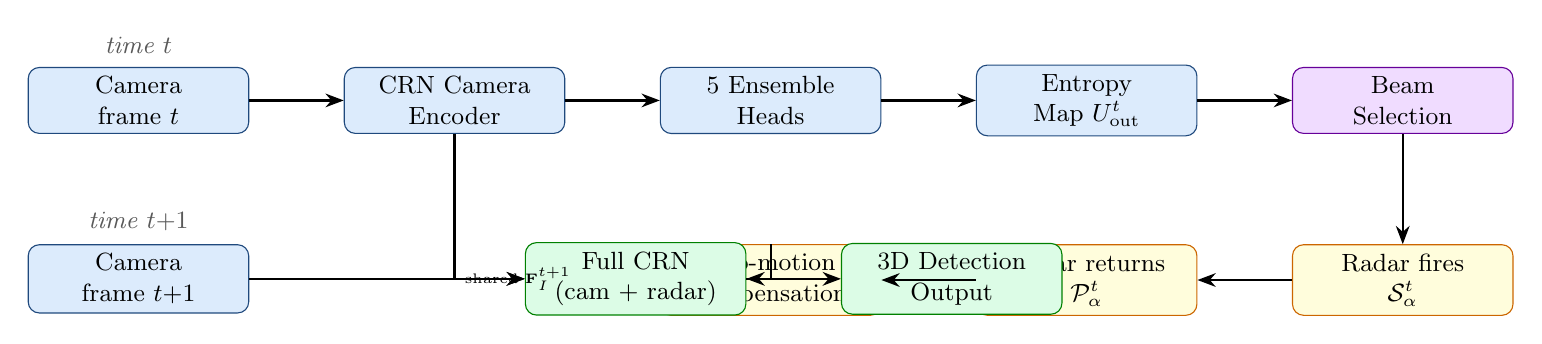
\begin{tikzpicture}[
  node distance=0.7cm and 1.2cm,
  box/.style={draw, rounded corners, minimum width=2.8cm, minimum height=0.8cm,
    align=center, font=\small},
  cambox/.style={box, fill=lightblue, draw=thesisblue},
  radarbox/.style={box, fill=lightyellow, draw=inprogressorange},
  fusebox/.style={box, fill=lightgreen, draw=donegreen},
  decbox/.style={box, fill=lightpurple, draw=plannedpurple},
  arr/.style={-Stealth, thick},
  timearr/.style={-Stealth, thick, dashed, gray}
]

% Frame t pipeline
\node[cambox] (cam_t) {Camera\\frame $t$};
\node[cambox, right=of cam_t] (enc_t) {CRN Camera\\Encoder};
\node[cambox, right=of enc_t] (ens_t) {5 Ensemble\\Heads};
\node[cambox, right=of ens_t] (ent_t) {Entropy\\Map $\Uout^t$};
\node[decbox, right=of ent_t] (sel_t) {Beam\\Selection};

% Radar
\node[radarbox, below=1.4cm of sel_t] (radar) {Radar fires\\$\beamset_\alpha^t$};
\node[radarbox, left=of radar] (returns) {Radar returns\\$\mathcal{P}_\alpha^t$};
\node[radarbox, left=of returns] (egocomp) {Ego-motion\\compensation};

% Frame t+1 pipeline
\node[cambox, below=1.4cm of cam_t] (cam_t1) {Camera\\frame $t{+}1$};
\node[fusebox, right=3.5cm of cam_t1] (crn_full) {Full CRN\\(cam + radar)};
\node[fusebox, right=of crn_full] (detect) {3D Detection\\Output};

% Arrows - frame t
\draw[arr] (cam_t) -- (enc_t);
\draw[arr] (enc_t) -- (ens_t);
\draw[arr] (ens_t) -- (ent_t);
\draw[arr] (ent_t) -- (sel_t);
\draw[arr] (sel_t) -- (radar);
\draw[arr] (radar) -- (returns);
\draw[arr] (returns) -- (egocomp);

% Arrows - frame t+1
\draw[arr] (cam_t1) -- (crn_full);
\draw[arr] (egocomp) |- (crn_full);
\draw[arr] (enc_t) |- node[right, font=\tiny]{shared $\FI^{t+1}$} (crn_full);
\draw[arr] (crn_full) -- (detect);

% Time annotations
\node[font=\small\itshape, color=thesisgray, above=0.05cm of cam_t] {time $t$};
\node[font=\small\itshape, color=thesisgray, above=0.05cm of cam_t1] {time $t{+}1$};

\end{tikzpicture}
\end{center}

\subsection{Why Fuse with $t+1$ and Not $t$}

\begin{center}
\renewcommand{\arraystretch}{1.3}
\begin{tabular}{lll}
  \toprule
  \textbf{Criterion} & \textbf{Fuse with $t$} & \textbf{Fuse with $t+1$} \\
  \midrule
  Temporal alignment & Poor (radar arrives after $t$) & Good (radar arrives near $t+1$) \\
  Spatial alignment & Requires motion compensation & Standard motion comp.\ \\
  Causal consistency & Beam based on $t$, fused with $t$ & Beam based on $t$, fused with $t+1$ \\
  Practical latency & Would require waiting for returns & Natural pipeline flow \\
  nuScenes analogy & --- & Multi-sweep accumulation \\
  \bottomrule
\end{tabular}
\end{center}

\begin{plainbox}
\textbf{Is it a problem that the beam was selected based on frame $t$ but
fused with frame $t+1$?}

No, for two reasons:
\begin{enumerate}
  \item Objects move slowly relative to the camera frame rate.
        A car at 50 km/h moves $\sim 1$\,m between frames at 12 Hz.
        The beam pointing toward that car at frame $t$ still covers it at frame $t+1$.
  \item The uncertainty map changes smoothly. A region that was uncertain at
        frame $t$ is almost always still uncertain at frame $t+1$.
        The beam selection from one frame is a good proxy for the next frame.
\end{enumerate}
This is actually a feature of the system: beam scheduling can run one frame
ahead of detection, providing a natural pipeline structure.
\end{plainbox}

% =============================================================================
\section{Experimental Phases}
\label{sec:phases}
% =============================================================================

\subsection{Phase 1 --- LSS Ensemble (Completed)}
\label{sec:phase1}

\begin{donebox}
  Phase~1 is complete. Camera-only LSS ensemble entropy outperforms random and
  uniform beam selection at every $\alpha$. Convergence at $\alpha^* =$ [fill]\%.
\end{donebox}

\paragraph{What it does.} Train a 5-member LSS ensemble on car BEV occupancy
(camera only). Compute entropy over the 5 predictions. Score beams by average
entropy. Select top-$K$ beams. Feed masked radar to CRN. Evaluate detection.

\paragraph{What it proves.} Camera perceptual uncertainty is a valid proxy for
beam utility. This establishes the core idea of the thesis.

\paragraph{Limitation.} Uses a weaker, separate model (LSS) instead of CRN itself.
Phase~2 addresses this.

\begin{algorithm}[H]
\caption{Phase~1: LSS Ensemble Beam Selection}
\label{alg:phase1}
\begin{algorithmic}[1]
\Require Camera images $\{I_n\}$, LSS ensemble $\{f^{(m)}\}_{m=1}^5$,
         full radar $\mathcal{P}$, fraction $\alpha$
\State \textbf{Uncertainty:} $\hat{p}^{(m)}\gets f^{(m)}(\{I_n\})$ for $m=1..5$
\State $\bar{p}(x,y)\gets\frac{1}{5}\sum_m\hat{p}^{(m)}(x,y)$
\State $\Uout(x,y)\gets-\bar{p}\log\bar{p}-(1-\bar{p})\log(1-\bar{p})$
\State \textbf{Beam selection:} $\mathcal{S}(\beam_i)\gets
       \frac{1}{|\mathcal{G}(\beam_i)|}\sum_{(x,y)\in\mathcal{G}(\beam_i)}\Uout(x,y)$
\State $\beamset_\alpha\gets\text{top-}K\text{ beams by }\mathcal{S}$
\State \textbf{Detection:} $\mathcal{P}_\alpha\gets\text{mask}(\mathcal{P},\beamset_\alpha)$
\State \Return $\mathrm{CRN}(\{I_n\},\mathcal{P}_\alpha)$
\end{algorithmic}
\end{algorithm}

\subsection{Phase 2 --- CRN-Internal Uncertainty (Next)}
\label{sec:phase2}

\begin{nextbox}
  Phase~2 replaces the external LSS ensemble with uncertainty signals from
  within CRN itself. Phase~2-A is the \textbf{core new contribution}.
  Phases~2-B and~2-C are ablation signals.
\end{nextbox}

\subsubsection{Phase 2-A: CRN Camera Ensemble Heads (Core)}

\begin{corebox}
\textbf{This is the primary Phase~2 contribution.}
Train 5 independent detection heads on the CRN camera branch output.
Compute output entropy from these heads. Select beams. Run full CRN with radar.
Same logic as Phase~1 but using CRN's own features.
\end{corebox}

The camera encoder runs once. 5 lightweight heads run in parallel on its output
(Eq.~\eqref{eq:cam_ensemble_heads}). Entropy is computed (Eq.~\eqref{eq:cam_entropy}).
Beams are selected (Eq.~\eqref{eq:topk}). Full CRN then runs with the
camera encoder output reused and masked radar added.

\subsubsection{Phase 2-B: Depth Distribution Entropy (Ablation)}

\begin{ablationbox}
This is an ablation signal, not the core method.
It tests whether the depth distribution entropy $\Udep$ (how spread-out CRN's
per-pixel depth estimate is) is a useful complementary signal to output entropy.
\end{ablationbox}

\begin{plainbox}
Recall that CRN predicts, for every pixel, a probability distribution over 112
possible depths (2\,m to 58\,m). When this distribution is flat, the camera
cannot determine depth at that pixel. We compute the Shannon entropy of this
distribution and project it to BEV as an alternative uncertainty map.

This is different from output entropy: a pixel may have confident depth
(low depth entropy) but still be uncertain about object class (high output entropy),
or vice versa. Comparing the two tells us which type of uncertainty is more
predictive of beam utility.
\end{plainbox}

\begin{equation}
  \Udep(u,v)
  = -\sum_{d=1}^{D}\DI(u,v,d)\log\DI(u,v,d)
  \;\in\;\bigl[0,\,\log 112\bigr]
  \label{eq:depth_entropy}
\end{equation}

Projected to BEV via the same Voxel Pooling as RVT:
\begin{equation}
  U_B(x,y) = \frac{1}{|\mathcal{F}(x,y)|}
  \sum_{(n,d,u,v)\in\mathcal{F}(x,y)}\Udep^{(n)}(u,v)
  \label{eq:depth_entropy_bev}
\end{equation}

\subsubsection{Phase 2-C: MFA Attention Weights (Ablation)}

\begin{ablationbox}
This is an ablation signal. It tests whether the MFA's learned modality
preference (how much it would rely on radar at each BEV location) can guide
beam selection. It is the weakest of the three signals because the attention
weights are partially unreliable when radar is absent (out-of-distribution input).
\end{ablationbox}

\begin{plainbox}
When we run CRN with no radar input, the MFA attention module still computes
weights over the (empty) radar features. These weights reflect where the model
\emph{would} rely on radar if it were present --- a spatial prior learned
from thousands of training scenes.

High radar attention at a BEV location means the model has learned
``I need radar here to make a good prediction.''
This is a beam selection candidate.

The limitation: since the radar input is zero (out-of-distribution for the MFA),
the weights are noisy compared to what they would be with real radar data.
The CRN paper shows the model was trained with random radar drop, so it
does not collapse completely, but this signal is less reliable than Phases~2-A and~2-B.
\end{plainbox}

\begin{equation}
  \Uatt(x,y)
  = \frac{1}{H}\sum_{h=1}^{H}\sum_{k=1}^{K} A_{h,\mathrm{radar},q(x,y),k}
  \label{eq:attention_uncertainty}
\end{equation}

\subsubsection{Phase 2 Summary}

\begin{center}
\renewcommand{\arraystretch}{1.3}
\begin{tabular}{lllll}
  \toprule
  & \textbf{2-A} & \textbf{2-B} & \textbf{2-C} & \\
  \textbf{Signal} & Output entropy & Depth entropy & Attn.\ weights
    & \textbf{Role} \\
  \midrule
  Type & Task-level semantic & Geometric & Learned & \\
  Source & 5 heads on CRN cam & Depth head & MFA layers & \\
  Radar absent? & Not needed & Not needed & Noisy & \\
  \textbf{Role} & \textcolor{corered}{\textbf{Core}} &
    \textcolor{plannedpurple}{Ablation} &
    \textcolor{plannedpurple}{Ablation} & \\
  \bottomrule
\end{tabular}
\end{center}

\subsection{Phase 3 --- Learned Beam Selection Policy (Future)}
\label{sec:phase3}

\begin{futurebox}
  Phase~3 replaces the heuristic beam score with a supervised MLP trained
  on pre-computed beam utility labels. It removes the greedy independence
  assumption by learning beam interactions from data.
\end{futurebox}

\paragraph{Marginal beam utility labels.}
\begin{equation}
  u_i(s)
  = \mathrm{mAP}(s,\{\beam_i\}) - \mathrm{mAP}(s,\emptyset)
  \label{eq:marginal_utility}
\end{equation}
Pre-compute offline for all 120 beams $\times$ 700 training scenes
$= 84{,}000$ CRN forward passes ($\approx 70$ GPU-hours, one-time).

\paragraph{Scorer network.}
Pool camera BEV features over each beam's angular sector:
\begin{equation}
  \mathbf{v}_i = \frac{1}{|\mathcal{G}(\beam_i)|}
    \sum_{(x,y)\in\mathcal{G}(\beam_i)}\Fbev_\mathrm{cam}(x,y)
  \label{eq:beam_pool_feat}
\end{equation}

Train a lightweight MLP: $\hat{u}_i = \mathrm{MLP}_\theta(\mathbf{v}_i)$
with MSE + pairwise ranking loss~\cite{burges2005learning}:
\begin{equation}
  \mathcal{L}
  = \frac{1}{N_B}\sum_i(\hat{u}_i-u_i)^2
  + \lambda_r\sum_{i\neq j}\max\!\bigl(0,-(u_i-u_j)(\hat{u}_i-\hat{u}_j)\bigr)
  \label{eq:scorer_loss}
\end{equation}

% =============================================================================
\section{Baselines}
\label{sec:baselines}
% =============================================================================

\begin{center}
\renewcommand{\arraystretch}{1.4}
\begin{tabular}{llp{6cm}l}
  \toprule
  \textbf{ID} & \textbf{Name} & \textbf{Rule} & \textbf{Status} \\
  \midrule
  B0 & Full Radar & All 120 beams. Upper bound.
    & \textcolor{donegreen}{\textbf{Done}} \\
  B1 & No Radar & Camera-only CRN. Lower bound.
    & \textcolor{donegreen}{\textbf{Done}} \\
  B2 & Random & $K$ random beams; avg.\ 10 seeds.
    & \textcolor{donegreen}{\textbf{Done}} \\
  B3 & Uniform & $K$ beams at equal angular spacing.
    & \textcolor{donegreen}{\textbf{Done}} \\
  B4 & Density & Top-$K$ beams by radar point count.
    & \textcolor{inprogressorange}{\textbf{Needed}} \\
  B5 & GT Oracle & Top-$K$ beams by GT object-centre count.
    & \textcolor{inprogressorange}{\textbf{Needed}} \\
  B6 & Phase~1 & LSS entropy (Section~\ref{sec:phase1}).
    & \textcolor{donegreen}{\textbf{Done}} \\
  \bottomrule
\end{tabular}
\end{center}

Density baseline: $\mathcal{S}_\mathrm{density}(\beam_i)
= |\{j:\mathrm{atan2}(y_j,x_j)\in\beam_i\}|$.
GT Oracle: $\mathcal{S}_\mathrm{oracle}(\beam_i)
= |\{k:\theta(\mathbf{c}_k)\in\beam_i\}|$.

% =============================================================================
\section{Additional Analyses}
\label{sec:additional}
% =============================================================================

\subsection{Convergence and Power Saving}
\begin{equation}
  \alpha^* = \inf\left\{\alpha:\mathrm{mAP}(\beamset_\alpha)
    \geq 0.99\cdot\mathrm{mAP}(\beamset_{1.0})\right\},
  \quad
  \mathrm{PS} = (1-\alpha^*)\times100\%
  \label{eq:convergence}
\end{equation}
AUC over the full curve: $\mathrm{AUC}=\sum_k\mathrm{mAP}(\alpha_k)\Delta\alpha_k$.

\subsection{Epistemic vs.\ Total Entropy (Ablation)}

\begin{ablationbox}
Compare $\Hent_\mathrm{total}$, $\Hent_\mathrm{epist}$, and $\Hent_\mathrm{aleat}$
as beam scores. Expected finding: \textbf{total entropy performs best} because
aleatoric camera uncertainty is still resolvable by radar.
$\Hent_\mathrm{aleat}$ alone should perform worst (negative control).
\end{ablationbox}

\subsection{Beam Width Sensitivity}
Test $\Delta\theta\in\{1^\circ,3^\circ,5^\circ,10^\circ\}$ at Phase~2-A,
$\alpha=0.2$.

\subsection{Weather Breakdown}
Evaluate under day/sunny, day/rainy, night.
Night hypothesis: $\Uout$ is uniformly high everywhere (camera degrades),
reducing beam selectivity advantage. Honest limitation to report.

\subsection{Cross-Class Generalisation}
Phase~1 trains on cars only. Report per-class AP for cars, trucks, pedestrians,
bicycles to assess generalisation.

% =============================================================================
\section{Dataset and Metrics}
\label{sec:dataset}
% =============================================================================

\textbf{nuScenes}~\cite{caesar2020nuscenes}: 6 cameras ($1600\times900$\,px),
5-channel radar accumulated over 6 sweeps, 10-class 3D boxes.
700/150/150 train/val/test. All evaluation on val set.

Beam fraction sweep:
$\alpha\in\{0.05, 0.10, 0.15, 0.20, 0.25, 0.30, 0.40, 0.50, 0.60, 0.75, 1.00\}$.

Metrics: mAP, Car AP (primary), NDS, mATE, mAVE.

% =============================================================================
\section{Timeline and Status}
\label{sec:timeline}
% =============================================================================

\begin{center}
\renewcommand{\arraystretch}{1.4}
\begin{tabular}{llll}
  \toprule
  \textbf{Phase} & \textbf{Task} & \textbf{Status} & \textbf{Duration} \\
  \midrule
  \multirow{4}{*}{\textbf{Ph.1}}
  & LSS 5-head ensemble trained & \textcolor{donegreen}{\textbf{Done}} & --- \\
  & Entropy scoring + beam mapping & \textcolor{donegreen}{\textbf{Done}} & --- \\
  & $\alpha$-sweep on val set & \textcolor{donegreen}{\textbf{Done}} & --- \\
  & Beats random + uniform confirmed & \textcolor{donegreen}{\textbf{Done}} & --- \\
  \midrule
  \multirow{2}{*}{\textbf{Baselines}}
  & Density (B4) & \textcolor{inprogressorange}{\textbf{Needed}} & 1--2 days \\
  & GT Oracle (B5) & \textcolor{inprogressorange}{\textbf{Needed}} & 1--2 days \\
  \midrule
  \multirow{5}{*}{\textbf{Ph.2-A}}
  & Add 5 ensemble heads to CRN camera branch & \textcolor{inprogressorange}{\textbf{Next}} & 3--4 days \\
  & Fine-tune heads on nuScenes train & \textcolor{inprogressorange}{\textbf{Next}} & 1--2 days \\
  & Output entropy $\to$ beam scoring & \textcolor{inprogressorange}{\textbf{Next}} & 2 days \\
  & Full $\alpha$-sweep + comparison & \textcolor{inprogressorange}{\textbf{Next}} & 3 days \\
  & Validate camera-only mAP vs CRN Table~8 & \textcolor{inprogressorange}{\textbf{Next}} & 1 day \\
  \midrule
  \multirow{3}{*}{\textbf{Ablations}}
  & Ph.2-B: depth entropy signal & \textcolor{plannedpurple}{\textbf{Planned}} & 3 days \\
  & Ph.2-C: MFA attention weights & \textcolor{plannedpurple}{\textbf{Planned}} & 3 days \\
  & Epist.\ vs total entropy comparison & \textcolor{plannedpurple}{\textbf{Planned}} & 2 days \\
  \midrule
  \multirow{4}{*}{\textbf{Ph.3}}
  & Pre-compute $u_i(s)$ labels ($\sim$70 GPU-hrs) & \textcolor{plannedpurple}{\textbf{Planned}} & 1--2 weeks \\
  & Train MLP beam scorer & \textcolor{plannedpurple}{\textbf{Planned}} & 1 week \\
  & Full evaluation & \textcolor{plannedpurple}{\textbf{Planned}} & 1 week \\
  & (Optional) End-to-end training & \textcolor{plannedpurple}{\textbf{Planned}} & 2 weeks \\
  \midrule
  \multirow{3}{*}{\textbf{Paper}}
  & Ablations + weather + qualitative figures & \textcolor{plannedpurple}{\textbf{Planned}} & 2 weeks \\
  & Writing & \textcolor{plannedpurple}{\textbf{Planned}} & 3 weeks \\
  & Revision + submission & \textcolor{plannedpurple}{\textbf{Planned}} & 1 week \\
  \bottomrule
\end{tabular}
\end{center}

% =============================================================================
\section{What We Have and What We Need}
\label{sec:summary}
% =============================================================================

\subsection*{What We Have}
\begin{itemize}[leftmargin=2em]
  \item[\textcolor{donegreen}{\textbf{v}}]
        nuScenes pipeline with beam masking (Eq.~\eqref{eq:masking})
  \item[\textcolor{donegreen}{\textbf{v}}]
        Pretrained CRN, verified on nuScenes val
  \item[\textcolor{donegreen}{\textbf{v}}]
        LSS deep ensemble (5 members), car class, camera-only
  \item[\textcolor{donegreen}{\textbf{v}}]
        Phase~1 results: entropy beats random/uniform at all $\alpha$
  \item[\textcolor{donegreen}{\textbf{v}}]
        Power-saving convergence at $\alpha^*=$ [fill value]
\end{itemize}

\subsection*{What We Need}
\begin{itemize}[leftmargin=2em]
  \item[\textcolor{inprogressorange}{\textbf{>}}]
        Baselines B4 (Density) and B5 (GT Oracle)
  \item[\textcolor{inprogressorange}{\textbf{>}}]
        Phase~2-A: 5 ensemble heads on CRN camera branch + results
  \item[\textcolor{plannedpurple}{\textbf{o}}]
        Ablations: Ph.2-B, Ph.2-C, epistemic vs total entropy
  \item[\textcolor{plannedpurple}{\textbf{o}}]
        Phase~3: beam utility labels + trained scorer
  \item[\textcolor{plannedpurple}{\textbf{o}}]
        Weather, beam-width, cross-class analyses
  \item[\textcolor{plannedpurple}{\textbf{o}}]
        Hero qualitative figure: 6 cams / uncertainty map / selected beams / detections
  \item[\textcolor{plannedpurple}{\textbf{o}}]
        All results tables filled in
\end{itemize}

% =============================================================================
% Bibliography
% =============================================================================
\newpage
\bibliographystyle{ieeetr}
\begin{thebibliography}{99}

\bibitem{haykin2006cognitive}
S.~Haykin,
``Cognitive radar: A way of the future,''
\emph{IEEE Signal Process.\ Mag.}, vol.~23, no.~1, pp.~30--40, 2006.

\bibitem{haykin2012cognitive}
S.~Haykin, Y.~Xue, and T.~N.~Davidson,
``Optimal waveform design for cognitive radar,''
in \emph{Proc.\ 42nd Asilomar Conf.}, pp.~3--7, 2008.

\bibitem{bell1993information}
M.~R.~Bell,
``Information theory and radar waveform design,''
\emph{IEEE Trans.\ Inf.\ Theory}, vol.~39, no.~5, pp.~1578--1597, 1993.

\bibitem{shannon1948mathematical}
C.~E.~Shannon,
``A mathematical theory of communication,''
\emph{Bell Syst.\ Tech.\ J.}, vol.~27, no.~3, pp.~379--423, 1948.

\bibitem{mackay1992information}
D.~J.~C.~MacKay,
``Information-based objective functions for active data selection,''
\emph{Neural Comput.}, vol.~4, no.~4, pp.~590--604, 1992.

\bibitem{houlsby2011bayesian}
N.~Houlsby, F.~Husz\'{a}r, Z.~Ghahramani, and M.~Lengyel,
``Bayesian active learning for classification and preference learning,''
\emph{arXiv:1112.5745}, 2011.

\bibitem{settles2009active}
B.~Settles,
``Active learning literature survey,''
Univ.\ Wisconsin, Tech.\ Rep.\ 1648, 2009.

\bibitem{kendall2017uncertainties}
A.~Kendall and Y.~Gal,
``What uncertainties do we need in Bayesian deep learning for computer vision?''
in \emph{Proc.\ NeurIPS}, pp.~5574--5584, 2017.

\bibitem{gal2016dropout}
Y.~Gal and Z.~Ghahramani,
``Dropout as a Bayesian approximation,''
in \emph{Proc.\ ICML}, pp.~1050--1059, 2016.

\bibitem{lakshminarayanan2017simple}
B.~Lakshminarayanan, A.~Pritzel, and C.~Blundell,
``Simple and scalable predictive uncertainty estimation using deep ensembles,''
in \emph{Proc.\ NeurIPS}, pp.~6405--6416, 2017.

\bibitem{depeweg2018decomposition}
S.~Depeweg, J.-M.~Hernandez-Lobato, F.~Doshi-Velez, and S.~Udluft,
``Decomposition of uncertainty in Bayesian deep learning,''
in \emph{Proc.\ ICML}, pp.~1189--1198, 2018.

\bibitem{sensoy2018evidential}
M.~Sensoy, L.~Kaplan, and M.~Kandemir,
``Evidential deep learning to quantify classification uncertainty,''
in \emph{Proc.\ NeurIPS}, pp.~3179--3189, 2018.

\bibitem{burges2005learning}
C.~J.~Burges \emph{et al.},
``Learning to rank using gradient descent,''
in \emph{Proc.\ ICML}, pp.~89--96, 2005.

\bibitem{kim2023crn}
Y.~Kim, J.~Shin, S.~Kim, I.-J.~Lee, J.~W.~Choi, and D.~Kum,
``CRN: Camera radar net for accurate, robust, efficient 3D perception,''
\emph{arXiv:2304.00670}, 2023.

\bibitem{kim2023craft}
Y.~Kim, S.~Kim, J.~W.~Choi, and D.~Kum,
``CRAFT: Camera-radar 3D object detection with spatio-contextual fusion transformer,''
in \emph{Proc.\ AAAI}, 2023.

\bibitem{nabati2021centerfusion}
R.~Nabati and H.~Qi,
``CenterFusion: Center-based radar and camera fusion for 3D object detection,''
in \emph{Proc.\ WACV}, pp.~1527--1536, 2021.

\bibitem{zhou2023bridging}
T.~Zhou, J.~Chen, Y.~Shi, K.~Jiang, M.~Yang, and D.~Yang,
``Bridging the view disparity between radar and camera features,''
\emph{IEEE Trans.\ Intell.\ Veh.}, vol.~8, no.~6, pp.~3124--3136, 2023.

\bibitem{philion2020lss}
J.~Philion and S.~Fidler,
``Lift, splat, shoot,''
in \emph{Proc.\ ECCV}, pp.~194--210, 2020.

\bibitem{li2023bevdepth}
Y.~Li \emph{et al.},
``BEVDepth: Acquisition of reliable depth for multi-view 3D object detection,''
in \emph{Proc.\ AAAI}, 2023.

\bibitem{li2022bevformer}
Z.~Li \emph{et al.},
``BEVFormer: Learning bird's-eye-view representation from multi-camera images,''
in \emph{Proc.\ ECCV}, pp.~1--18, 2022.

\bibitem{caesar2020nuscenes}
H.~Caesar \emph{et al.},
``nuScenes: A multimodal dataset for autonomous driving,''
in \emph{Proc.\ CVPR}, pp.~11621--11631, 2020.

\bibitem{he2016deep}
K.~He, X.~Zhang, S.~Ren, and J.~Sun,
``Deep residual learning for image recognition,''
in \emph{Proc.\ CVPR}, pp.~770--778, 2016.

\bibitem{lin2017feature}
T.-Y.~Lin, P.~Doll\'{a}r, R.~Girshick, K.~He, B.~Hariharan, and S.~Belongie,
``Feature pyramid networks for object detection,''
in \emph{Proc.\ CVPR}, pp.~2117--2125, 2017.

\bibitem{lang2019pointpillars}
A.~H.~Lang \emph{et al.},
``PointPillars: Fast encoders for object detection from point clouds,''
in \emph{Proc.\ CVPR}, pp.~12697--12705, 2019.

\bibitem{qi2017pointnet2}
C.~R.~Qi, L.~Yi, H.~Su, and L.~J.~Guibas,
``PointNet++: Deep hierarchical feature learning on point sets,''
in \emph{Proc.\ NeurIPS}, pp.~5105--5114, 2017.

\bibitem{yan2018second}
Y.~Yan, Y.~Mao, and B.~Li,
``SECOND: Sparsely embedded convolutional detection,''
\emph{Sensors}, vol.~18, no.~10, p.~3337, 2018.

\bibitem{huang2021bevdet}
J.~Huang, G.~Huang, Z.~Zhu, and D.~Du,
``BEVDet: High-performance multi-camera 3D object detection,''
\emph{arXiv:2112.11790}, 2021.

\bibitem{zhu2021deformable}
X.~Zhu, W.~Su, L.~Lu, B.~Li, X.~Wang, and J.~Dai,
``Deformable DETR,''
in \emph{Proc.\ ICLR}, 2021.

\bibitem{yin2021centerpoint}
T.~Yin, X.~Zhou, and P.~Kr\"{a}henb\"{u}hl,
``Center-based 3D object detection and tracking,''
in \emph{Proc.\ CVPR}, pp.~11784--11793, 2021.

\end{thebibliography}
\end{document}
